% status: 100
% chapter: Azure

\title{Report: Resource Orchestration Using Azure Service Fabric }


\author{Tolu Agunbiade}
\affiliation{%
	\institution{Indiana University}
	\city{Bloomington} 
	\state{IN} 
	\postcode{47408}
        \country{USA}}
\email{toagun@iu.edu}


% The default list of authors is too long for headers}
\renewcommand{\shortauthors}{G. v. Laszewski}


\begin{abstract}
The need to modularize software gave rise to the Service Oriented
Architecture (SOA) paradigm of the early 1990s. Traditionally, 
it was
conceived to solve complex enterprise architecture problems with the
goals of facilitating usability. However the needs of the enterprise
have evolved into enabling continuous evolution, ensuring the
efficiency of the software development team, reducing cost, increasing
software portability and ensure a flexible technology architecture
especially for the enterprise to avoid technology
lock-in. Furthermore, as companies mature and grow, applications today
need to be adaptable to changes quickly, be platform agnostic to
reduce the risk of introducing latest technologies, and to scale
seamlessly to multiple geographic locations, datacenters or cloud to
intake new users or systems. These business needs gave rise to
Microservices. Microservices is essentially an improvement over 
the Service
Oriented Architecture approach to software deployment and management.
In Microservices, software applications are
designed to be modular and to communicate using defined protocols
and interfaces. The fact that these 
services are decoupled
and broken down therefore necessitates the need for management and
orchestration to ensure the component parts work together to deliver
on the business objective. This paper will discuss the use of Azure
Service Fabric to orchestrate the resources or services in a
Microservices architecture set up to ensure business objectives are
realized.

\end{abstract}

\keywords{hid-sp18-501, Microservices, Service-Oriented Architecture,
Azure Service Fabric, Resource Manager, Orchestration}


\maketitle


\section{Introduction}

Since the earliest days of developing applications for the web, the
most widely used enterprise application architecture has been one that
packages all the application's server-side components into a single
unit~\cite{hid-sp18-501-infoq}. Traditionally, such applications which
are usually said to be in a {\bf Service-Oriented Architecture} are built
to consist of several components to manage the different aspects of
the application which is made up mainly of a client-side user
interface, a database and server-side application. This approach to
application development is often called the monolithic
architecture. The monolithic application was easy to maintain as the
developers only needed to build and deploy an updated version of the
server-side application to make any alterations to the
system~\cite{hid-sp18-501-mulesoft}. However, monolithic applications
are often tightly coupled together as the application evolves making
it difficult to understand dependencies and to isolate services for
scaling or maintenance~\cite{hid-sp18-501-trello}.
 
In a marked difference from monolithic application development,
Microservices architecture approach incorporate designs
that loosely couple different application but that jointly implement
common business capabilities~\cite{hid-sp18-501-microservicesio}. 
By incorporating this design principle, a typical microservice
architecture enables the continuous delivery and deployment of large and
complex applications~\cite{hid-sp18-501-researchgate}. 
Before cloud computing became hugely popular as it
is now, a lot of enterprise applications were built on-premise and
were not developed to be cloud-ready. However, the cloud presents a
number of advantages such as high availability and scalability that a
lot of the legacy applications that are on-premise cannot take
advantage of~\cite{hid-sp18-501-springer}. Microservices is a form of
architecture that is native to the cloud, meaning applications
developed as microservices are ready to be deployed to the cloud. In
microservices, the underlying codes are small ensuring developer
productivity. As stated earlier, each independednt service in a 
microservice-architected environment can be independently deployed.
~\cite{hid-sp18-501-infoq}.

The modern approach to microservices deployment is to deploy each
microservice in a container. Containerization or container-based
virtualization is an operating-system level method for managing 
distributed applications without launching an entire virtual
machine for each application~\cite{hid-sp18-501-techtarget}. Instead,
multiple isolated systems called containers are used to host the
different microservices.

Despite the many promises of Microservices, there are still some
obvious drawbacks. For example in a Microservices environment,
developers must deal with the additional complexities of creating and
maintaining distributed
systems~\cite{hid-sp18-501-patterns}. Deploying microservices also
requires centralized monitoring, logging and
alerting~\cite{hid-sp18-501-challenges} or simply put,
orchestration. For the microservices architecture to also achieve
loose coupling, each microservice is usually designed to have its own
database~\cite{hid-sp18-501-patterns}.

The need for orchestration is further heightened when we consider that
a single application can be modularized by being developed as a
microservice and each service can then be deployed on separate
containers. This application hyper-modularization is an important
reason why orchestration is key to achieving the business objective in
a microservices architecture.


\section{Orchestrating Microservices}
Using orchestrators for appplications is essential if the application
is based on microservices or is split across multiple
containers~\cite{hid-sp18-501-dotnet}. As you build an application
that uses microservices, decisions would have to be made about how the
different microservices interact. Orchestration is the traditional way
of handling interactions between different services in a microservices
architecture. A typical microservices architecture consists of the
management module, service discovery ability and an API gateway to
manage the entry point for clients that are calling the services. {\
bf Figure 1}
shows a typical Microservices Architecture.

\begin{figure*}[!ht]
  \centering\includegraphics[width=\columnwidth]{images/fig1.pdf}
  \caption{A Typical Microservices Architecture~\cite{hid-sp18-501-fig1}}
\label{f:architecture}
\end{figure*}

Since there are multiple services and applications in a microservices, 
avoiding
service inconsistencies and distruption means that the
multiple constituent parts must be somewhat orchestrated
~\cite{hid-sp18-501-opensource}. Orchestration in microservices 
architecture is the means by which service distruption and 
inconsistencies are avoided by employing monitoring tools to
manage and if necessary scale the various multiple resources 
in the microservices set up~\cite{hid-sp18-501-opensource}. 
There are many tools available 
that might enable this. For
containerized microservices, open source tools like Kubernetes
can be
used for orchestration~\cite{hid-sp18-501-onfido}. Alternatively, for
non-containerized microservices, other tools such as OpenStack may be
used for orchestrating the microservices
components~\cite{hid-sp18-501-rackspace}.

Another important tool that can be used for microservices
orchestration is the Microsoft Azure Service Fabric.



\section{Microsoft Azure Service Fabric}
Azure Service Fabric (ASF) is a Platform-as-a-Service offering
designed to facilitate the development, deployment and management of
highly scalable and customiuzable applications for the Microsft Azure
Cloud platform~\cite{hid-sp18-501-definition}. By design, ``Service Fabric 
enables
building and managing scalable and reliable applications composed of
microservices that run at high density on a shared pool of machines,
which is referred to as a cluster''~\cite{hid-sp18-501-overview}. 
Azure Service Fabric is designed to allow and build microservices that are
``distributed, scalable, stateless, and that could run in containers''.
It also provides
comprehensive application management capabilities to ``provision,
deploy, monitor, upgrade/patch, and delete deployed applications
including containerized microservices''~\cite{hid-sp18-501-overview}.

Azure Service Fabric's key capabilities are described in {\bf Figure 2}:

\begin{figure*}[!ht]
  \centering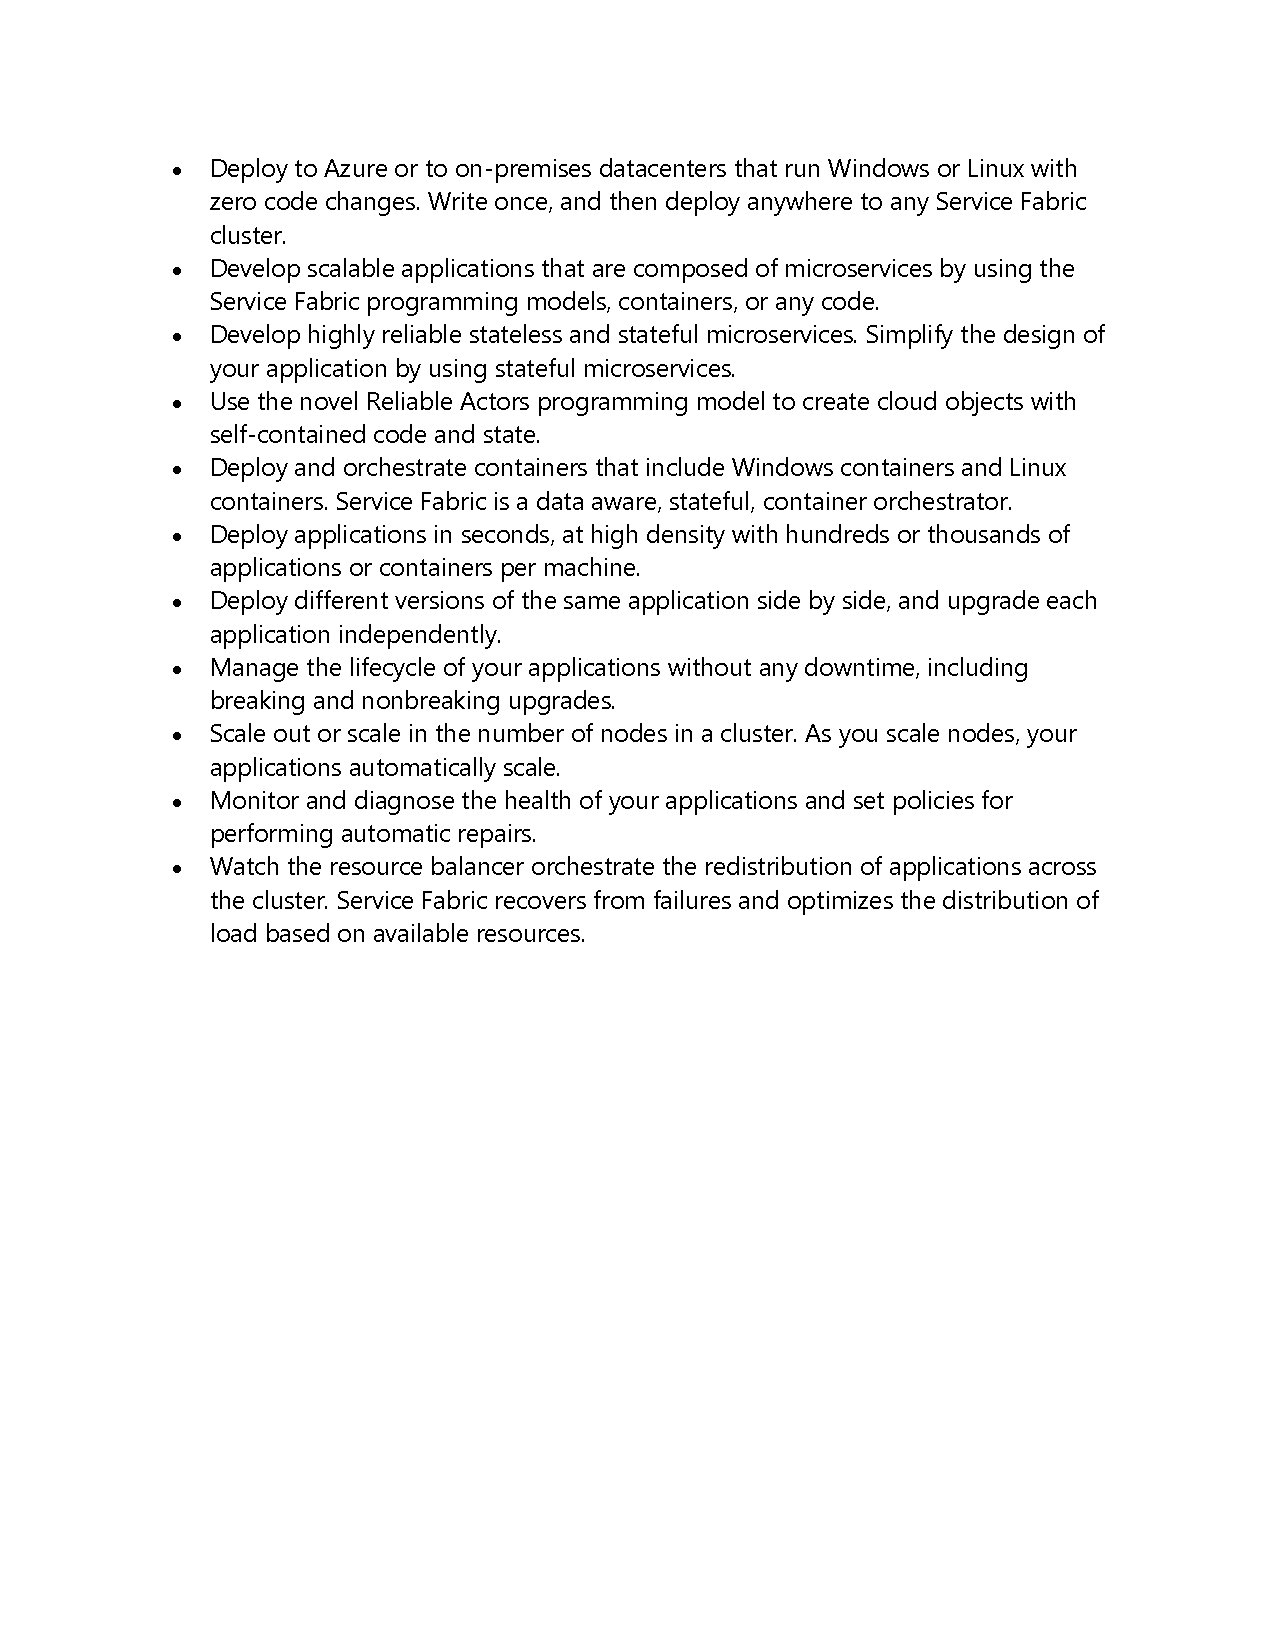
\includegraphics[width=\columnwidth]{images/fig2.pdf}
  \caption{Azure Service Fabric Capabilities~\cite{hid-sp18-501-overview}}
\label{f:architecture}
\end{figure*}


\section{Resource Orchestration with Azure Service Fabric}
Much like the music conductor in an orchestra, {\bf ``Orchestrator} is the 
general term for a piece of software that
helps administrators manage the deployment of distributed
services''~\cite{hid-sp18-501-fig2and3}. Orchestrators work by allowing 
services to act in a certain
way based on pre-defined triggers. For example, 
``orchestrators are what
swing into action when a machine fails, or a workload or service
terminates for some unexpected reason''~\cite{hid-sp18-501-fig2and3}. 
Depending 
on configuration, manufacturer and the archiecture, ``most 
orchestrators do more than
just deal with failure, such as helping with new deployments, handling
upgrades, and dealing with resource consumption, but all are
fundamentally about maintaining some desired state of configuration in
the environment''~\cite{hid-sp18-501-fig2and3}.
 
Orchestrators must have the ability to enable administrators
preconfigure settings to manage the microservices
under its care.

The primary means of enabling orchestration within Service Fabric is
through the Cluster Resource Manager.

The Service Fabric incoporates many systems and tool, however
``The Service Fabric 
Cluster Resource Manager is one of the System
Services within Service Fabric and is automatically started up within
each cluster''~\cite{hid-sp18-501-fig2and3}.  
{\bf Figure 3} shows the three major parts of the Resource Manager's job.

\begin{figure*}[!ht]
  \centering
\includegraphics[width=\columnwidth]{images/fig3.pdf}
  \caption{The Resource Manager's Job~\cite{hid-sp18-501-fig2and3}}
\label{f:architecture}
\end{figure*}


\section{The Service Fabric Cluster Resource Manager}

\subsection{Service Fabric Resource Manager vs Network Load Balancer}

In traditional N tier web-apps there was always some notion of a {\bf Load
Balancer}, usually referred to as a Network Load Balancer (NLB) or an
Application Load Balancer (ALB) depending on where it sits in the
networking stack. In these architectures the job of load balancing is
to make sure that all of the different stateless front-end machines or
the different machines in the cluster receive (roughly) the same
amount of work. There are many ways to achieve this, ``from sending each
different call to a different server, to session pinning/stickiness,
to actual estimation and call allocation based on its expected cost
and current machine load''~\cite{hid-sp18-501-fig2and3}.

The reason for this architecture was at best the mechanism for
ensuring that the web tier remained roughly
balanced~\cite{hid-sp18-501-fig2and3}.  Strategies for balancing the
data tier were completely different and depended on the data storage
mechanism, usually centering around data sharding, caching, database
managed views and stored procedures, etc
~\cite{hid-sp18-501-fig2and3}.

Some of the approaches we've discussed are interesting, but most 
importabrly
``the Service Fabric
Resource Manager is not anything like a network load balancer or a
cache''~\cite{hid-sp18-501-fig2and3}. By default, ``NLB ensures 
that the front
ends are balanced by moving traffic to where the services are running,
the Service Fabric Resource Manager on the other hand takes a completely 
different approach, 
fundamentally, Service Fabric moves services to where they make the
most sense''~\cite{hid-sp18-501-fig2and3}. This can be, for example,
nodes which are ``currently cold because the services which are there
are not doing a lot of work at the moment''~\cite{hid-sp18-501-fig2and3}.
It could also be away ``from a node which is about to be upgraded or
which is overloaded due to a spike in consumption of the services
which were running on it''~\cite{hid-sp18-501-fig2and3}. Because it is
responsible for moving services around (not delivering network traffic
to where services already are), the Service Fabric Resource Manager is
more versatile and also contains additional capabilities for
controlling where and how services are moved.

\subsection{General Architecture}
The ability for Service Fabric Resource Manager 
to execute on th tasks as described in the last section depends on the 
amount of information that is available to the Resource Manager.
~\cite{hid-sp18-501-fig2and3}.  It has to
know which services currently exist and their current (or default)
amount of resources that a service is consuming. The Resource Manager
is also ``designed to know the capacity of the nodes in the cluster, and
in essence the resources available in the whole cluster plus whatever
resources remaining on a particular node''
~\cite{hid-sp18-501-fig2and3}. In today's application development, the
resources consumed by a service can vary with time. In typical 
deployments for many services,
there could be {\bf ``real} resources like memory
and disk consumption that are commonly used across many different
types of services, as well as resources that only a particular service
care about~\cite{hid-sp18-501-fig2and3}''.  Another challenge is 
that in most cases ``the owners and operators of the cluster are
different from the service authors, or at a minimum are
the same people wearing different hats''~\cite{hid-sp18-501-fig2and3}. 
For example in the case a service needs to be developed, it is possible
to ``know a few things about what is required in terms of
resources and how the different components should ideally be
deployed''~\cite{hid-sp18-501-fig2and3}. However for the same service
different tools might be required to manage a live-site incident. In
addition, the cluster and the service are designed to be elastic, that is
``the number of nodes in the cluster can grow and
shrink, nodes of different sizes can come and go, and services can
change their resource allocation, and be created and
removed''~\cite{hid-sp18-501-fig2and3}.  The importance of microservices
necessitates a lot of high-touch (such as upgrades).  These high-touch
operations can in essence trigger unexpected failures. By design, the
Service Fabric Resource Manager ``stores information about the overall
microservices cluster, and the requirements of the different
micoservices services''~\cite{hid-sp18-501-fig2and3}. To satisfy this
design requirement, ``Service
Fabric typically deploys two agents, a Resource Manager that runs on
individual nodes in order to aggregate local resource consumption
information, and another agent which is a centralized, fault-tolerant
Resource Manager service that aggregates all of the information about
the services and the cluster and reacts to changes based on the
desired state configuration of the cluster and
service''~\cite{hid-sp18-501-fig2and3}.

{\bf Figure 4} shows the deployment of the two Resource Manager agents in
Azure Service Fabric.

\begin{figure*}[!ht]
  \centering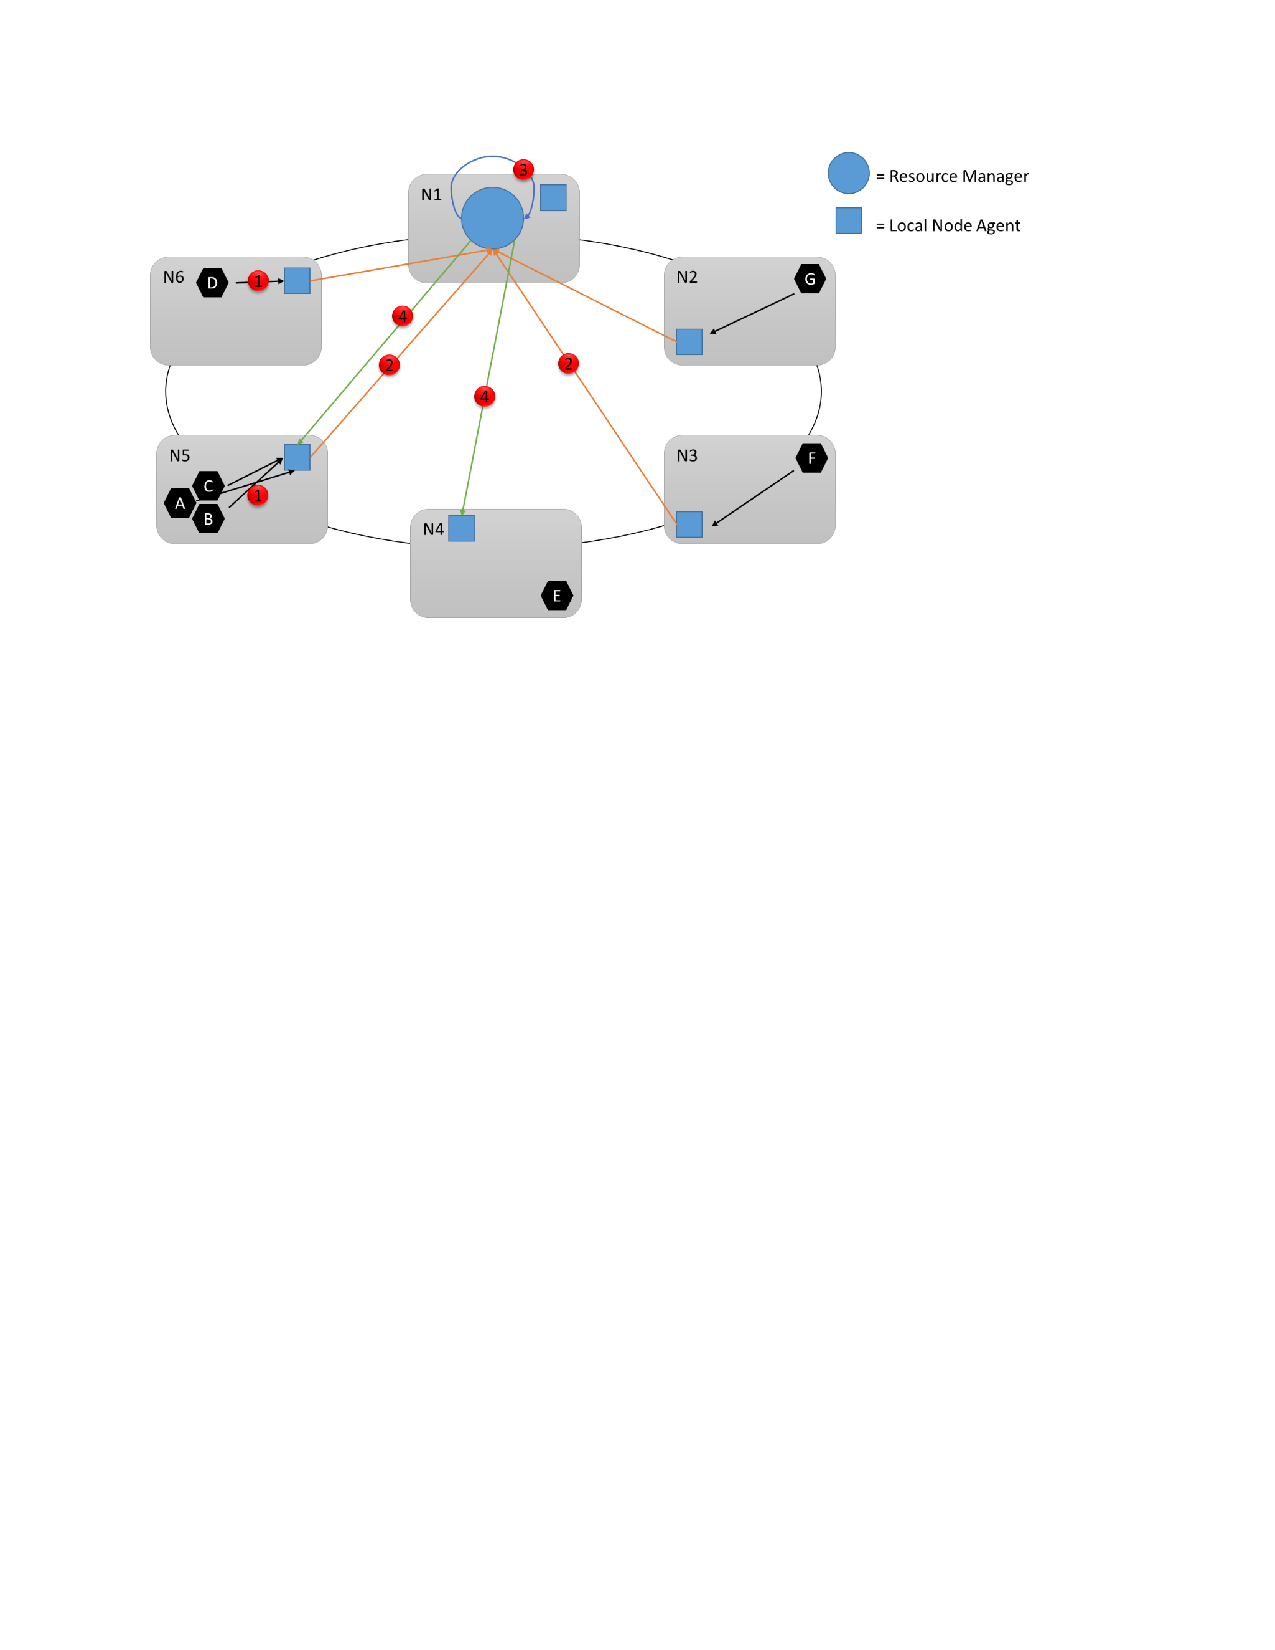
\includegraphics[width=\columnwidth]{images/fig4.pdf}
  \caption{General Resource Manager Function~\cite{hid-sp18-501-fig2and3}}
\label{f:architecture}
\end{figure*}

During a typical runtime, ``there could be some changes in the amount of
resources services consume, some service failures, or some nodes join
and leave the cluster''~\cite{hid-sp18-501-fig2and3}.  All the changes
on a specific node are aggregated and periodically sent to the central
Resource Manager service (1,2) where they are aggregated again,
analyzed, and stored.  Every few seconds that central service looks at
all the changes and determines if there are any actions necessary
(3). The Resource Manager is designed to also be able to move services
to new nodes detected in the cluster. It could also notice that a node
is overloaded, or that certain services have failed (or been deleted),
freeing up resources on other nodes.

{\bf Figure 5} shows how the Resource Manager reacts to the scenario we
painted earlier.

\begin{figure*}[!ht]
  \centering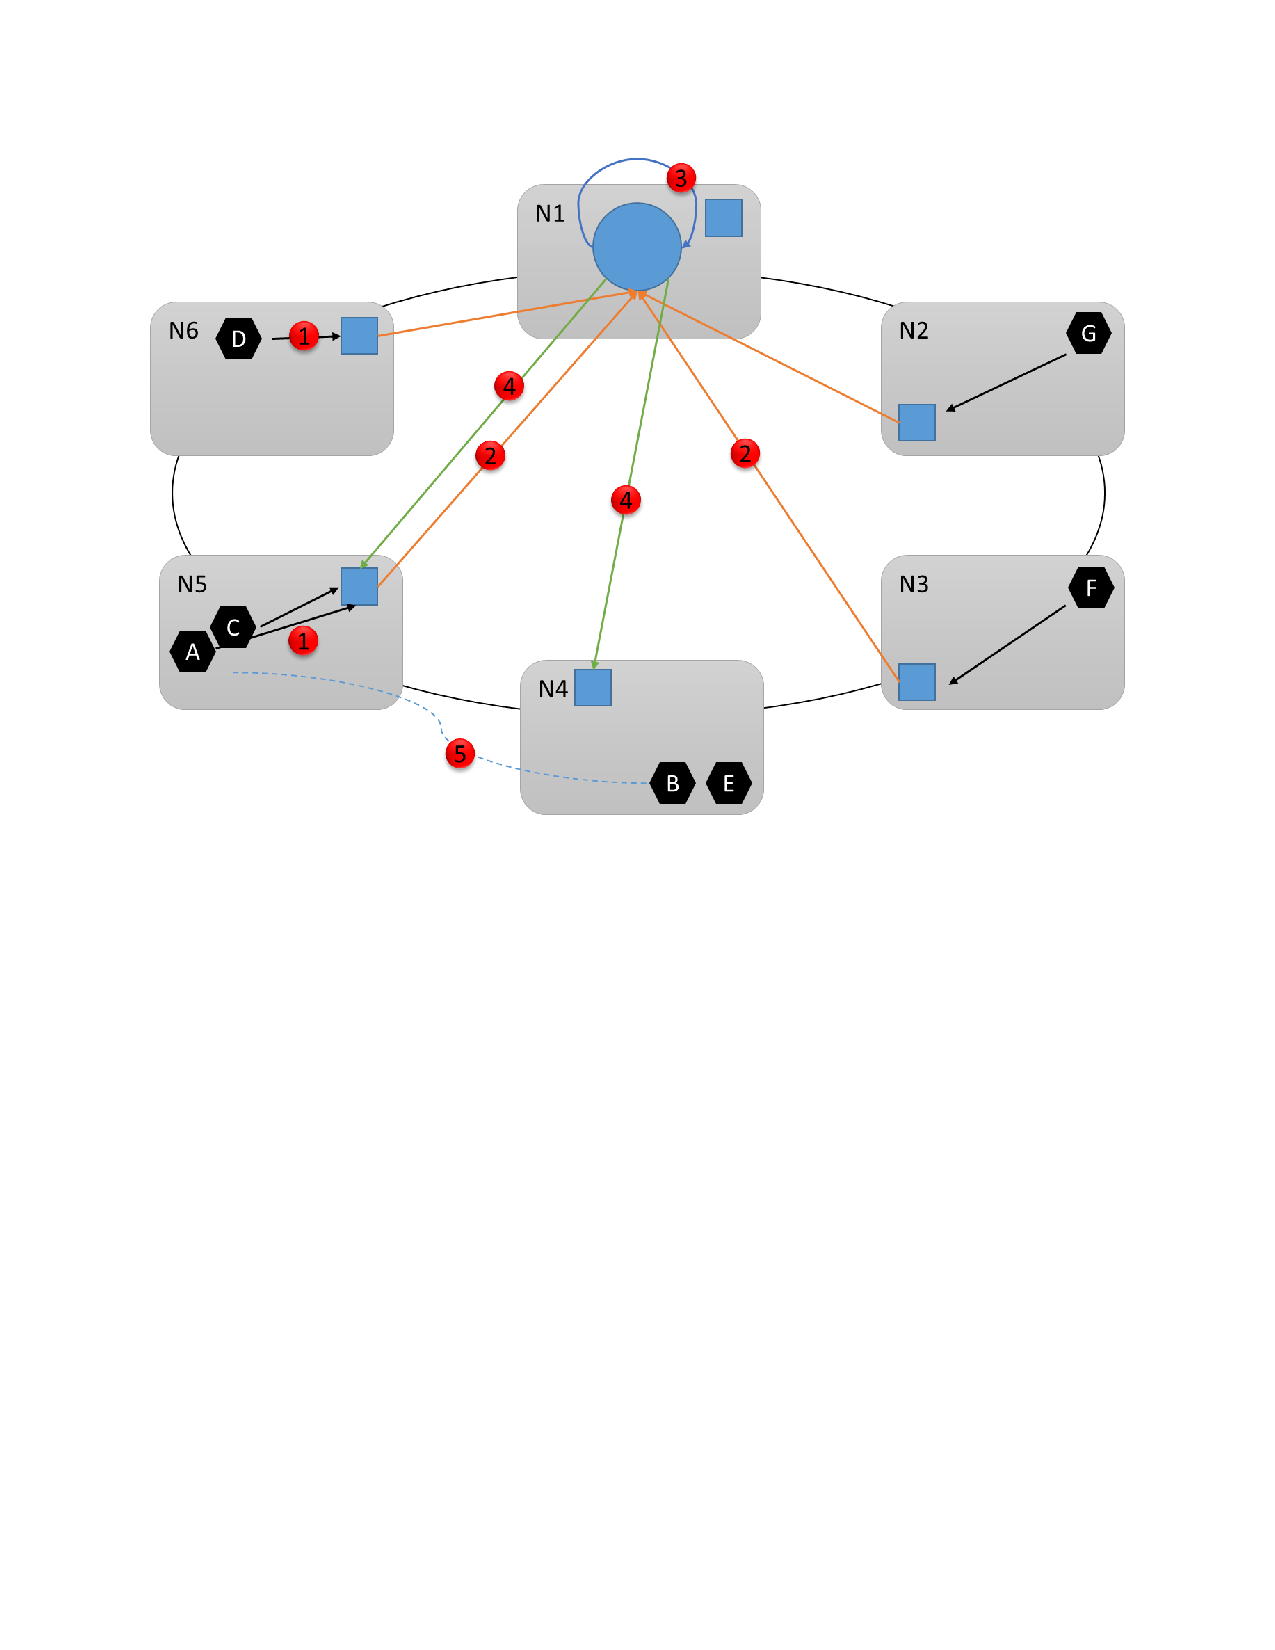
\includegraphics[width=\columnwidth]{images/fig5.pdf}
  \caption{Resou
rce Manager Reconfigures the Cluster~\cite{hid-sp18-501-fig2and3}}
\label{f:architecture}
\end{figure*}

As soon as the Resource Manager determines that changes are necessary
it coordinates with other system services (in particular the Failover
Manager) to make the necessary changes. Then the change requests are
sent to the appropriate nodes (4). In this case, we ``presume that the
Resource Manager noticed that Node 5 was overloaded, and so decided to
move service B from N5 to N4''~\cite{hid-sp18-501-fig2and3}. 
At the end of the reconfiguration (5),
the cluster looks like this what we have in {\bf Figure 5}

\section{Resource Management Mechanism}

\subsection{Fault Domains}
In a distributed architecture such as aim a microservice a fault
domain is any area of coordinated failure. ``A single machine'' in a cluster
represents a ``fault domain since it can fail for many reasons''
~\cite{hid-sp18-501-description}. 
Furthermore, a collection of
machines in the same virtual network or sharing the same power source
are also in a fault domain~\cite{hid-sp18-501-description}.

In setting up a cluster, a lot of attention is required for the
possible areas of failure. Given this, the Resource Manager's fault 
domains should be set
up in a way that Service Fabric can automatically and smartly determine and
triage where or how to place the services in the cluster in case of a
failure~\cite{hid-sp18-501-fig2and3}.

\subsection{Upgrade Domains}
The Resource Manager makes use of Upgrade Domains to help Service Fabric
understand the cluster layout so as to proactively manage failures. 
Upgrade Domains define areas (sets of
nodes, really) that will go down at the same time during an upgrade.

Upgrade Domains are usually defined by policy;
whereas Fault Domains are rigorously defined by the areas of
coordinated failures (and hence usually the hardware layout of the
environment). Furthermore, ``Upgrade Domains are not
hierarchical, they are more like a simple tag than a hierarchy''
~\cite{hid-sp18-501-fig2and3}.

The advantages of having a large number of upgrade domains is that
each stage of the cluster upgrade is granular and localized and
therefore affects a small set of nodes or microservices. This results
in fewer services having to move at a time, introducing less churn
into the system and overall improving reliability (since less of the
service will be impacted by any issue).  The disadvantage of having a
large number of ``upgrade domains is that Service Fabric verifies the
health of each Upgrade Domain as it is upgraded and ensures that the
Upgrade Domain is healthy before moving on to the next Upgrade
Domain'' and ``the goal of this check is to
ensure that services have a chance to stabilize and that their health
is validated before the upgrade proceeds, so that any issues are
detected''~\cite{hid-sp18-501-fig2and3}.  

There are also disdvantages for not having enough upgrade domains.
The disadvantage is most significant during an upgrade to an updgared
domain. In that case, it is possible that a substantial portion
of the cluster is down and unavailable. A cluster with 3 upgrade domain 
has a third of its
capacity unavailable if one of the domains is ongoing an upgrade. 
The Resource Manager architecture allows for limitless number of fault or 
upgrade domains
and the inter-relationships are not constrained
~\cite{hid-sp18-501-description}. Common structures that 
are 1:1 ratio (where each
unique fault domain maps to its own upgrade domain as well) an Upgrade
Domain per Node (physical or virtual OS instance), and a {\bf striped} or
{\bf matrix} model where the Fault Domains and Upgrade Domains form a
matrix with machines usually running down the diagonal.

Typically if a Service Fabric cluster is deployed on Azure, 
``Service Fabric
automatically defines the fault and upgrade domains and it 
just pick up the environment information from
Azure''~\cite{hid-sp18-501-description}. Azure also allows the 
Service Fabric admin
to ``pick the number of required domains''. In Azure both the fault and
upgrade domain information look like a {\bf single level} view, but it
really is ``encapsulating information from lower layers of the Azure
stack and just presenting the logical fault and upgrade domains from
the user's perspective''~\cite{hid-sp18-501-fig2and3}.

A point of note though. If the cluster is being set up manually, (or
just want to try running a particular topology on the development
machine) then the fault domain and upgrade information has to be
explicitly provided.

\subsection{Capacity Management}
Irrespective of the technology platform, orchestrators are designed to
manage the consumption of resources in any kind of cluster. Resource
optimization ensures that no nodes are hot (leading to resource
contention and poor performance) nor cold (wasted
resources). Orchestrators are also designed to ensure that clusters
resources are always-on.

To guarantee that resources are always-on, resources are represented
by Metrics in Service Fabric. In Service Fabric, ``Metrics are the units 
by which any
logical or physical resource is described or exposed''
~\cite{hid-sp18-501-fig2and3}. Examples of ``metrics are
{\bf WorkQueueDepth} or {\bf MemoryInMb}''~\cite{hid-sp18-501-description}. 
Again in Service Fabric, ``Metrics are different from
constraints and node properties in that node properties are generally
static descriptors of the nodes themselves, whereas metrics are about
physical resources that services consume when they are running on a
node''~\cite{hid-sp18-501-description}.  So a property would be something
like HasSSD and could be set to true or false, but the amount of space
available on that SSD (and consumed by services) would be a metric
like {\bf DriveSpaceInMb}. By design, ``capacity on the node would set the
{\bf DriveSpaceInMb} to the amount of total non-reserved space on the
drive, and services would report how much of the metric they used
during runtime''~\cite{hid-sp18-501-fig2and3}.

If all resource balancing are turned off, Service Fabric's Resource
Manager would still be able to ensure that no node ended up over its
capacity (unless the cluster as a whole was too full). Capacities are
the mechanism that Service Fabric uses to understand how much of a
resource a node has, from which we subtract consumption by different
services (more on that later) in order to know how much is left. The
Service Fabric Resource Manager represents capacity and consumption
service levels in terms of metrics~\cite{hid-sp18-501-description}.

During runtime, the Resource Manager tracks how much of each resource
is present on each node (defined by its capacity) and how much is
remaining (by subtracting any declared usage from each service).  The
tracking information is used by Service Fabric Resource Manager ``to
determine how to triage replicas to ensure nodes capacity are not over
utilized''~\cite{hid-sp18-501-description}.

In the case of dynamic load changes, replica nodes actually become invalid 
given that the ``combined usage of all of the replicas
and instances on that node exceeds that node's capacity''
~\cite{hid-sp18-501-description}. 
When this happens,
Service Fabric resource management ``automatically kicks in and gets the
node back below capacity by moving one or more of the replicas or
instances on that node to different nodes while minimizing the cost 
of all the movements in resource usage terms''~\cite{hid-sp18-501-description}.

\subsection{Cluster Capacity}
This section will examine how Service Fabric keeps the overall cluster
from performing over capacity. The design principle to achieve this
is to build in controls that prevent excessive capacity utilization. 
By default, ``the first of the controls is to prevent the creation
of new workloads that would cause the cluster to become full''
~\cite{hid-sp18-501-fig2and3}.

Consider a case where a stateless service is created with some
workloads.  For this service, let's say that it cares about some
resource (let’s say DiskSpace) and that by default it is going to
consume 5 units of DiskSpace for every instance of the service and
we'll like to create 3 instances of the service. This scenario
requires 15 units of DiskSpace in the cluster to be able to replicate
the service instances.  Again, by design ``Service Fabric will 
continually
calculate the overall capacity and consumption of each metric, so that
it can easily make the determination and reject the create service
call if there's insufficient space''~\cite{hid-sp18-501-fig2and3}.

Note that since the ``requirement is only that there be 15 units
available, this space could be allocated in different ways, it could
be one remaining unit of capacity on 15 different nodes, for example,
or three remaining units of capacity on 5 different nodes, 
etc''~\cite{hid-sp18-501-description}. 
When there is no sufficient capacity on three different nodes, Service
Fabric will ``reorganize the services already in the cluster in order to
make room on the three necessary nodes''~\cite{hid-sp18-501-description}. 
This reorganization is almost
always possible ``unless the whole cluster is almost entirely full,
however it can take some time to complete, potentially delaying the
start of the service instances''~\cite{hid-sp18-501-description}.

Additional cluster management capacity is also built into the Resource
Manager. For this scenario, Service Fabric enables the ability to
optionally reserve additional buffers to default node capacity. In the
current architecture, buffer ``is specified globally per metric for
all nodes via the ClusterManifest and the value picked for the
reserved capacity will be a function of which resources the services
are more constrained on, as well as the number of fault and upgrade
domains in the cluster''~\cite{hid-sp18-501-description}. Generally,
allowing for more fault and upgrade domains means that a ``lower
number of buffered capacity can be picked, since a smaller amount of
your cluster is to be unavailable during upgrades and failures''
~\cite{hid-sp18-501-description}.

\subsection{Placement Policies}
There are many different additional rules that are important
especially if a Service Fabric cluster is spanned across geographies, 
for example in multiple datacenters or Azure regions, ``or if the
environment spans multiple areas of geopolitical control''
~\cite{hid-sp18-501-placement}. Cofiguring this is possible by using the ``node 
properties and placement constraints
mentioned earlier''~\cite{hid-sp18-501-placement}. It is noteworthy that,
``just like placement constraints, placement policies can be configured
on a per-service basis'' as described in {\bf Figure 6} below.

\begin{figure*}[!ht]
  \centering
\includegraphics[width=\columnwidth]{images/fig6.pdf}
  \caption{Placement Policy Config Examples~\cite{hid-sp18-501-placement}}
\label{f:architecture}
\end{figure*}


Multiple Invalid or Required domains can be configured on a single
service, however the other two (preferred domains and domain
distribution) are only configurable once per service.

\subsubsection{Throttles}
In some cases, there can be distruption to the clusters
even when the resource manager is correctly configured. 
In this case, the Resource Manager will try its best to fix
everything, but in times like a backstop so that the cluster itself
has a chance to stabilize (the nodes which are going to come back come
back, the network conditions health themselves, corrected bits get
deployed) might have to be considered. To resolve situations like this, 
the Resource Manager makes use of throttles. Caution must be applied in 
the use of throttles though
as they are considered {\bf big hammers} and they should only be used after 
there is an undersatanding of the amount of
concurrent work that the cluster can execute. 
By default, the Resource Manager includes the
following default throttles:


- {\bf GlobalMovementThrottleThreshold}: This controls the
  total number of movements in the cluster over some time
  (defined as the
  {\bf GlobalMovementThrottleCountingInterval}, value in seconds)

- {\bf MovementPerPartitionThrottleThreshold}: This controls
  the total
  number of movements for any service partition 
  over some time (the
  {\bf MovementPerPartitionThrottleCountingInterval}, 
  value in seconds).


\subsubsection{Defragmentation}
In the examples we have considered so far, we have discussed balancing
in the context terms of load distribution in a cluster that is 
ensuring that loads in a cluster are equally utilized by all the
nodes. Architecting Service Fabric this way guarantees that no local
failure takes down the whole cluster.  However, the Service Fabric
Resource Manager also support defragmentation ``which is another way to
manage utilization in a cluster''~\cite{hid-sp18-501-defrag}. 
In general, defragmentation implies
that Service Fabric consolidates ``utilization instead of distributing
utilization of a metric across the cluster''~\cite{hid-sp18-501-defrag}.

Why defragmentation? When loads in a cluster is evenly distributed
amongst the nodes, the direct implication is therefore that at least
some of the resources at the node is used up; up to 75 to 95 percent
at a time.

Just like file creation or access could get slowed down if a
computer's hard disk was fragmented and could be sped up by
defragmenting the drive, defragmentation metrics can be configured to
have the Resource Manager proactively try to condense the load of the
services into fewer nodes so that there is (almost) always room for
even large services, enabling them to be created quickly.

In the Resource Manager configuration, the ``defragmented and normal
metrics can be mixed in the same cluster and the Resource Manager will
consolidate the layout to allow as much of the
defragmentation metrics as it can while at the same time to spread out the
rest''~\cite{hid-sp18-501-defrag}. The results in this case will depend 
on the ``number of balancing
metrics compared to the number of defragmentation metrics and their
weights''~\cite{hid-sp18-501-description}.


\section{Conclusion}
We have explored the mechanisms built in Azure Service Fabric 
Resource Manager to enable orchestrating 
microservices.

Increasingly, winning enterprise operating models require agility and
scalability across regulatory, compliance and business constraints on
global scale and at a much more frequent pace than we’ve ever
witnessed. The implication of this is that the underlying technology
architecture that supports a business must also be equally adaptable
to the rapid changes required of the operating models.

Microservices architecture enables the business to run multiple
loosely coupled but related services on the enterprise technology
stack. The rapid changes required of businesses and the
\textit{loosely-coupled} nature of microservice then requires a carefully
managed orchestration.

Azure Service Fabric is a Microsoft microservices technology offering
that enables enterprises meet the business objectives outlined
above. The Service Fabric Resource Manager enables enterprises to
exercise tight control and orchestrate resources in their Service
Fabric-based microservices. The Resource Manager enforces policies,
improve utilization, and get carbon-based life forms out of the
critical path when reacting to failures, managing processes like
upgrades, and trying to game out capacity and load scenarios in the
Service Fabric cluster.


\begin{acks}

  The authors would like to thank Dr.~Gregor~von~Laszewski for his
  support and suggestions to write this paper.

\end{acks}

\bibliographystyle{ACM-Reference-Format}
\bibliography{report}
